\documentclass{report}

\usepackage{apalike}
\usepackage{graphicx}

\title{replace title}
\author{replace author}
\date{replace date}

\begin{document}
\maketitle
\tableofcontents
\listoffigures

\chapter{Introduction}

\chapter{Executive Summary}
\section{Planning}
\subsection{Approach}
\subsection{Scope}
\subsection{Objectives}
\section{Methodology}
\subsection{Information Gathering}
\subsection{System Attacks}
\section{Summary of Findings}

\chapter{Key Findings}
\section{Auction Site}
This section covers the vulnerabilities found with the user-facing auction site.
\subsection{Path Traversal}
\subsubsection{Security Implications / Risk Level}
Path traversal allows for arbitrary file read across the system, for any files readable by the apache user (www-data). This is dangerous as it could potentially leak sensitive company data, as well as user data. If combined with other vulnerabilities, such as incorrect permissions on log files, it is possible to achieve Remote Code Execution through malicious log read/write.\\
Overall, the execution of this exploit is trivial, and the repercussions are potentially serious but not disasterous. Due to this, the risk level of this exploit is evaluated to be \textbf{medium}.
\subsubsection{Cause of Vulnerability}
The vulnerability is caused by the method used to retrieve and display image files on the website. Instead of directly referencing the image file through the 'src' field on an 'img' HTML tag, a PHP script is instead used to include the file.\\ 
While using PHP include scripts may not normally be dangerous, the file name to be retrieved can be edited by the user, allowing them to easily select which file should be displayed. A lack of filter/extension whitelist makes this even more potent.
\subsubsection{Steps to Replicate}
\begin{itemize}
		\item Firstly the inspect element tool in Mozilla Firefox was used to inspect an image, revealing the image URL (Fig. 3.1).
		\item The image URL could then be opened, showing the ASCII representation of the binary content for the image file (Fig. 3.2).
		\item Finally, the URL parameter 'file' could be replaced with a file path, allowing for arbitrary file read. In this example, the ../ operator was used to go up directories until root, and then the /etc/passwd file was navigated to (Fig. 3.3).
\end{itemize}
\begin{figure}
	\centering
	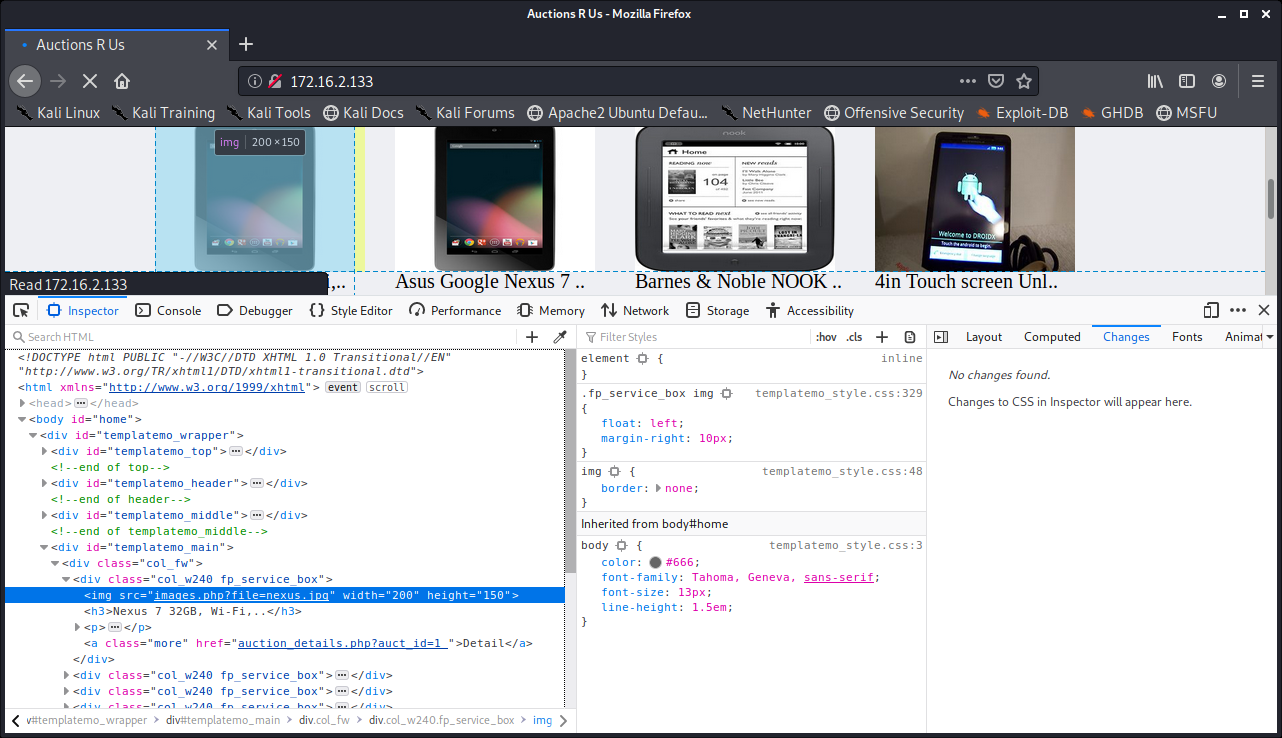
\includegraphics[scale=0.4]{img/pathtraversal1.png}
	\caption{Inspecting the image}
\end{figure}
\begin{figure}
	\centering
	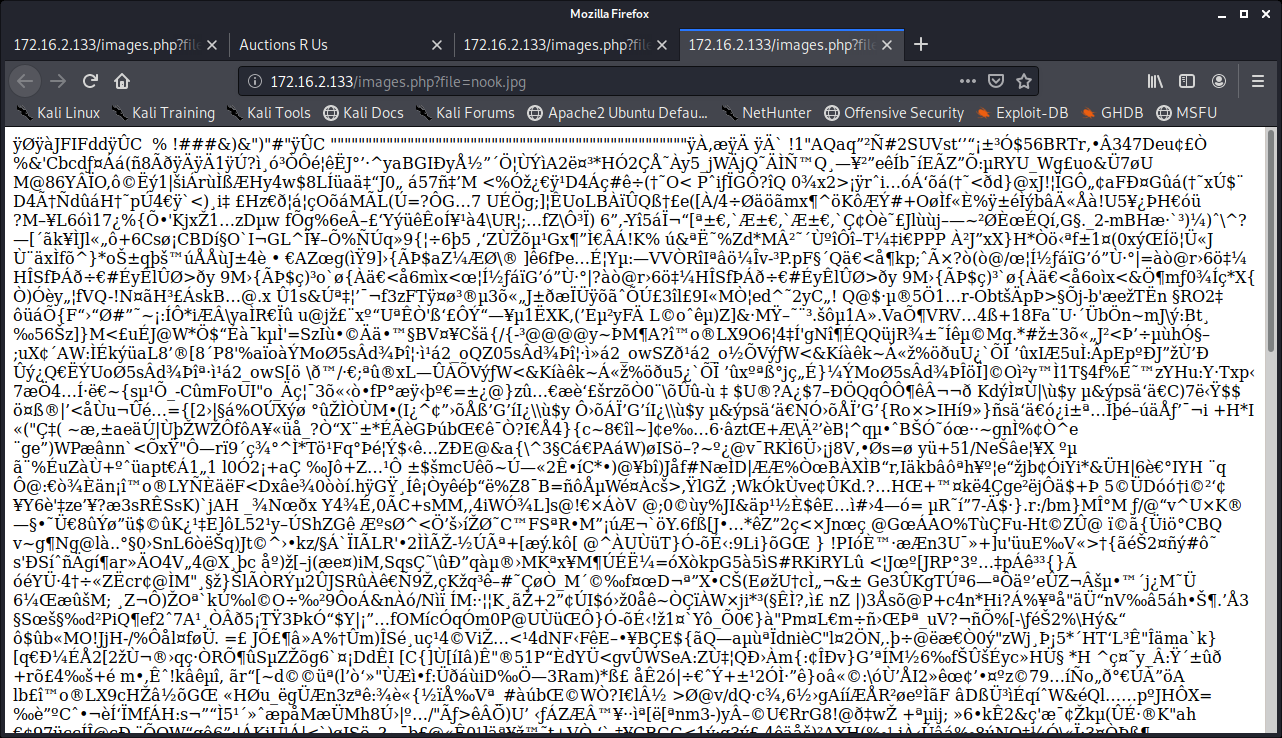
\includegraphics[scale=0.4]{img/pathtraversal2.png}
	\caption{Viewing the image contents}
\end{figure}
\begin{figure}
	\centering
	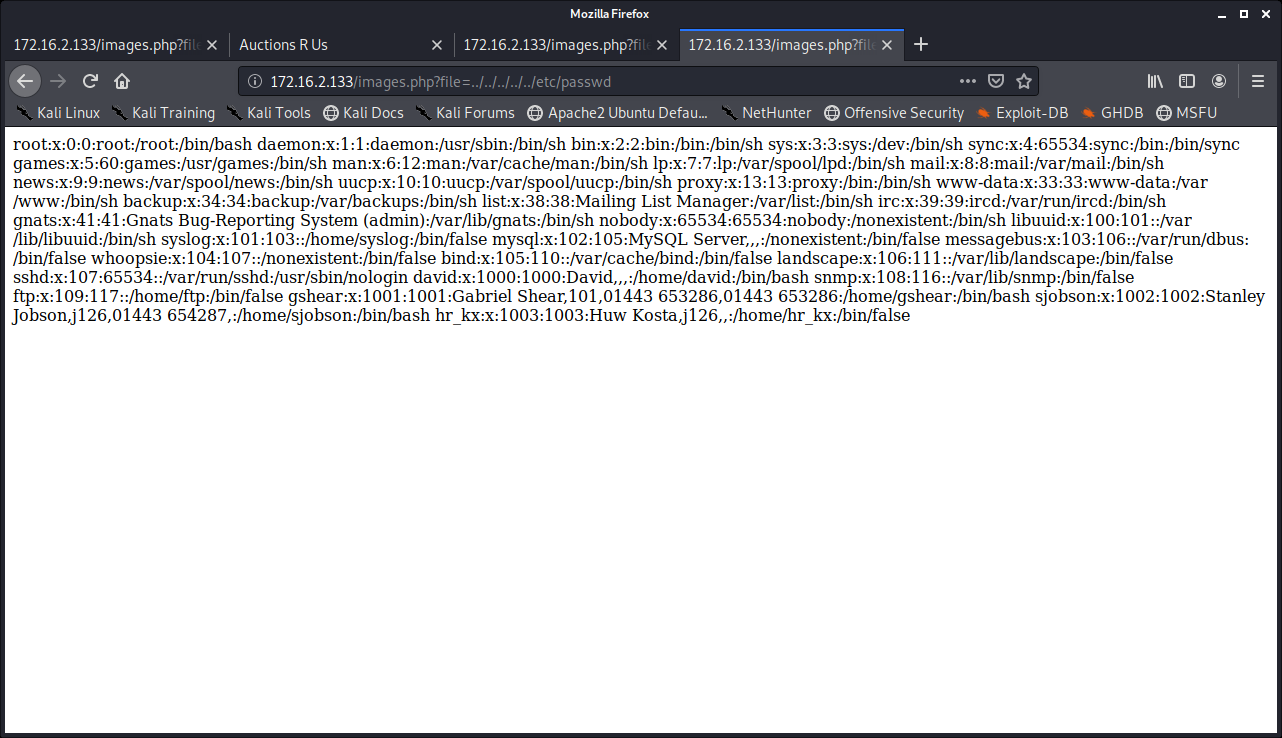
\includegraphics[scale=0.4]{img/pathtraversal3.png}
	\caption{Exploiting the file read}
\end{figure}
\pagebreak
\subsection{SQL Injection}
\subsubsection{Security Implications / Risk Level}
SQL injection is a blanket term covering any kind of unintended user control over the SQL queries interacting with a database. This can manifest in many forms, such as:
\begin{itemize}
	\item Authentication bypass, where SQL queries can be modified to bypass authentication checks such as login forms.
	\item Union injection, where the UNION keyword in SQL can be used to access data from other columns, tables, and databases.
	\item Error based injection, where SQL errors are intentionally created in order to gain information about the database.
	\item Blind injection, where queries that return TRUE or FALSE can be used to gain information about the database.
\end{itemize}
From the testing done, the website appears to be vulnerable to both authentication bypass, allowing attackers to log in to accounts, and blind injection, allowing for full read access across the database.\\
The execution of these exploits are relatively easy with the use of tools like SQLmap, and the repercussions can be very serious, allowing attackers to log in to administrator accounts as well as reading any user/auction data from the database. Due to this, the risk level of this exploit is evaluated to be \textbf{high}.
\subsubsection{Cause of Vulnerability}
SQL injection vulnerabilities are a result of allowing unsanitised user input in to SQL queries. Sanitising SQL queries involves removing any kind of dangerous character from the input, such as quotation marks (single and double) and comment tags. If this is not done, attackers are able to modify queries in specific ways to allow them to perform SQL injection.\\
One example of this would be performing an authentication bypass injection. A normal query may use a query like:
\begin{verbatim}
SELECT * FROM users WHERE username = '$inputname' AND password = 
'$inputpass';
\end{verbatim}
If an attacker enters something like ' OR 1=1\# in to the username field, the query becomes:
\begin{verbatim}
SELECT * FROM users WHERE username = '' OR 1=1#;
\end{verbatim}
Which will pick the first username from the table and sign the attacker in.
\subsubsection{Steps to Replicate}
\begin{itemize}
	\item For initial testing of SQL injection, a basic authentication bypass was used. The payload ' OR 1=1-- - was entered in to the username field (Fig. 3.4), which subsequently allowed access to the 'David' account, giving use of the admin panel as well (Fig. 3.5).
\end{itemize}
\pagebreak
\begin{figure}
	\centering
	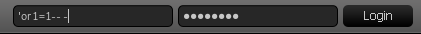
\includegraphics[scale=1]{img/sqli1.png}
	\caption{Authentication bypass SQLi}
\end{figure}
\begin{figure}
	\centering
	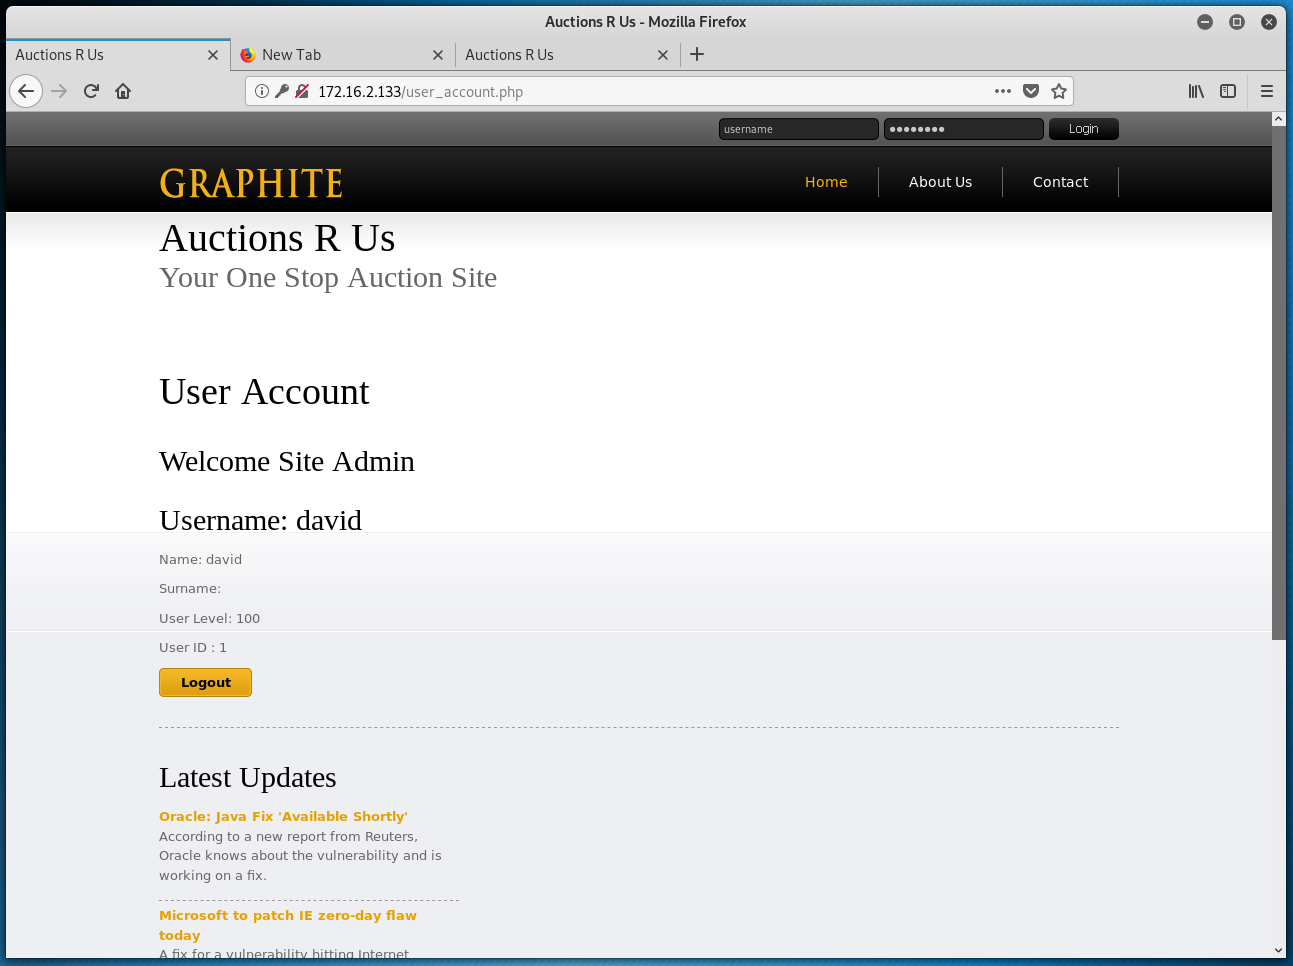
\includegraphics[scale=0.4]{img/sqli2.png}
	\caption{Admin panel access gained}
\end{figure}
\subsection{Weak Authentication}
\subsubsection{Security Implications / Risk Level}
\subsubsection{Cause of Vulnerability}
\subsubsection{Steps to Replicate}
script used to bruteforce the cookies
\section{SRV1}
\section{SRV2}
\section{Ubuntu Client}

\chapter{Recommendations}
\section{Auction Site}
\section{SRV1}
\section{SRV2}
\section{Ubuntu Client}

\chapter{Conclusion}

\chapter{References}


\end{document}